% \section{\KSe\ according to Evangelos}

The \KSe\ % (KSe)
reads:
 \beq
  u_t=(u^2)_x-u_{xx}- u_{xxxx} \, ,
  \label{eq:KS0}
 \eeq

 We assume periodic boundary conditions on the $x\in [0,2\pi \tilde{L}]$
 interval:
 \beq
   u(x+2\pi\tilde{L},t)=u(x,t) \, ,
 \eeq
 which allows a Fourier series expansion:
 \beq
  u(x,t)=\sum_{k=-\infty}^{+\infty} a_k (t) e^{ i k x / \tilde{L}} \, .
  \label{eq:Fourier}
 \eeq
 Since $u(x,t)$ is real,
 \beq
  a_{k}=a^*_{-k} \, .
  \label{eq:a*}
 \eeq
 Substituting \refeq{eq:Fourier} into \refeq{eq:KS} we get:
 \beq
  \dot{a}_k=(k/\tildeL)^2\left(1-(1/\tildeL)^2 k^2\right)a_k
        + i (k/\tildeL)  \sum_{m=-\infty}^{+\infty}a_m a_{k-m} \, .
  \label{eq:Fcoef}
 \eeq

 From \refeq{eq:Fcoef} we notice that $\dot{a}_0=0$ and thus $a_0$ is an integral
 of the equations or, from \refeq{eq:Fourier}, the average of the solution $\int dx u(x,t)$
 is a constant. Due to galilean invariance we may set $a_0=0$ without loss of generality
 and we only have to compute $a_k$'s with $k\geq 1$. % Explain this in detail somewhere.

 Truncating the infinite tower of equations by setting $a_k=0$ for $k>d$, using the identity $a_{-k}=a^*_k$ and splitting the
 resulting equations into real and imaginary part by setting $a_k=b_k+i c_k$, we have

 \bea
  \dot{b}_k & = & \left(\frac{k}{\tildeL}\right)^2\left(1- \left(k/\tildeL\right)^2 \right)b_k  \continue
    & & - \frac{k}{\tildeL} \left(\sum_{m=1}^{k-1}c_m b_{k-m}+\sum_{m=k+1}^{N}c_m b_{m-k}
                    -\sum_{m=1}^{N-k}c_m b_{k+m} \right)  \continue
    & & - \frac{k}{\tildeL} \left(\sum_{m=1}^{k-1}b_m c_{k-m}-\sum_{m=k+1}^{N}b_m c_{m-k}
                    +\sum_{m=1}^{N-k}b_m c_{k+m} \right)
  \label{eq:tmp:b-Trunc}
 \eea
 \bea
   \dot{c}_k & = & \left(\frac{k}{\tildeL}\right)^2\left(1- \left(k/\tildeL\right)^2 \right)c_k  \continue
    & & - \frac{k}{\tildeL}\left( \sum_{m=1}^{k-1}c_m c_{k-m}-\sum_{m=k+1}^{N}c_m c_{m-k}
                    -\sum_{m=1}^{N-k}c_m c_{k+m} \right)    \continue
    & & + \frac{k}{\tildeL} \left(\sum_{m=1}^{k-1}b_m b_{k-m}+\sum_{m=k+1}^{N}b_m b_{m-k}
                    +\sum_{m=1}^{N-k}b_m b_{k+m} \right)
   \label{eq:tmp:c-Trunc}
 \eea
 where now only terms $c_{k},b_{k}$ with $0<k<d$ appear. Observe
 \beq
    \sum_{m=1}^{N-k}c_m b_{k+m} = \sum_{m=k+1}^{N}b_m c_{m-k}\,,
 \eeq
 \etc and thus \refeq{eq:tmp:b-Trunc} and \refeq{eq:tmp:c-Trunc} simplify to
  \bea
  \dot{b}_k & = & \left(\frac{k}{\tildeL}\right)^2\left(1- \left(k/\tildeL\right)^2 \right)b_k  \continue
    & & - \frac{k}{\tildeL} \left(\sum_{m=1}^{k-1}c_m b_{k-m}-2\sum_{m=1}^{N-k}c_m b_{k+m} \right)  \continue
    & & - \frac{k}{\tildeL} \left(\sum_{m=1}^{k-1}b_m c_{k-m}+2\sum_{m=1}^{N-k}b_m c_{k+m} \right)
  \label{eq:b-Trunc}
 \eea
 \bea
   \dot{c}_k & = & \left(\frac{k}{\tildeL}\right)^2\left(1- \left(k/\tildeL\right)^2 \right)c_k  \continue
    & & - \frac{k}{\tildeL}\left( \sum_{m=1}^{k-1}c_m c_{k-m}-2\sum_{m=1}^{N-k}c_m c_{k+m} \right)  \continue
    & &  +\frac{k}{\tildeL}\left( \sum_{m=1}^{k-1}b_m b_{k-m}+2\sum_{m=1}^{N-k}b_m b_{k+m} \right)\,.
   \label{eq:c-Trunc}
 \eea

 To calculate the matrix of variations $A_{ij} \equiv \frac{\partial v_i(x)}{\partial x_j}$  we need to consider the four matrices $\frac{\partial \dot{b}_k}{\partial b_j},\frac{\partial \dot{b}_k}{\partial c_j},\frac{\partial \dot{c}_k}{\partial b_j},\frac{\partial \dot{c}_k}{\partial c_j}$. We begin with
 \bea
    \frac{\partial \dot{c}_k}{\partial c_{j}}  =
        \left(\frac{k}{\tildeL}\right)^2\left(1- \left(k/\tildeL\right)^2 \right) \delta_{kj}
            - \frac{k}{\tildeL}\frac{\partial}{\partial c_j}\left( \sum_{m=1}^{k-1}c_m c_{k-m}-2\sum_{m=1}^{N-k}c_m c_{k+m} \right) \,.
 \eea
 Concider the second term:
 \bea
    - \frac{k}{\tildeL}\frac{\partial}{\partial c_j}\left( \sum_{m=1}^{k-1}c_m c_{k-m}-2\sum_{m=1}^{N-k}c_m c_{k+m} \right) & = &
        - \frac{k}{\tildeL} \sum_{m=1}^{k-1} \left(\delta_{m,j} c_{k-m}+c_m \delta_{k-m,j} \right) \continue
                        & & + 2 \frac{k}{\tildeL}\sum_{m=1}^{N-k} \left(\delta_{m,j} c_{k+m}+c_m \delta_{k+m,j}\right)
 \eea
 We need to consider two cases separately:
 \begin{itemize}
    \item $k\leq j$
        \bea
             -\frac{k}{\tildeL}\frac{\partial}{\partial c_j}\left( \sum_{m=1}^{k-1}c_m c_{k-m}-2\sum_{m=1}^{N-k}c_m c_{k+m} \right) & = &
                    -\frac{k}{\tildeL}( 0+0 ) + 2\frac{k}{\tildeL} (c_{k+j} + c_{j-k}) \continue
                & = &   2 \frac{k}{\tildeL} (c_{k+j}-c_{k-j})
        \eea
    \item $k > j$
        \bea
             -\frac{k}{\tildeL}\frac{\partial}{\partial c_j}\left( \sum_{m=1}^{k-1}c_m c_{k-m}-2\sum_{m=1}^{N-k}c_m c_{k+m} \right) & = &
                    -\frac{k}{\tildeL}(c_{k-j} + c_{k-j} ) + 2\frac{k}{\tildeL} (c_{k+j}  + 0 ) \continue
                & = &  2 \frac{k}{\tildeL} (c_{k+j}-c_{k-j})
        \eea
 \end{itemize}
 and thus
 \beq
    \frac{\partial \dot{c}_k}{\partial c_{j}} =  \left(\frac{k}{\tildeL}\right)^2\left(1- \left(k/\tildeL\right)^2 \right) + 2 \frac{k}{\tildeL} (c_{k+j}-c_{k-j})
 \eeq

 Following the above procedure
 \beq
    \frac{\partial \dot{c}_k}{\partial b_{j}} =  2 \frac{k}{\tildeL} ( b_{k+j}+b_{k-j} )\,,
 \eeq
 \beq
    \frac{\partial \dot{b}_k}{\partial b_{j}} =  \left(\frac{k}{\tildeL}\right)^2\left(1- \left(k/\tildeL\right)^2 \right)\delta_{kj} - 2 \frac{k}{\tildeL} (c_{k+j} + c_{k-j}) \,,
 \eeq
 \beq
    \frac{\partial \dot{b}_k}{\partial c_{j}} = 2 \frac{k}{\tildeL} (b_{k+j}-b_{k-j}) \,.
 \eeq

\PC{Vaggelis, you might want to include some of the text commented out here
    into your thesis}
% In terms of the system size $ 2\pi L$, the only length scale available,
% the dimensions of terms in \refeq{ks} are
% $ %\[
% [x]=L
% $, $%\,,\quad
% [t]=L^2
% $, $%\,,\quad
% [u]=L^{-1}
% $, $%\,,\quad
% [\nu]=L^2
% \,.
% $ %\]
% What is the non-dimensional ``Rayleigh'' number for the
% \KS\ system?
%  Scaling out the ``viscosity'' $\nu$
% \[
% x \to x \nu^{\frac{1}{2}}
% \,,\quad
% t \to t \nu
% \,,\quad
% u \to u \nu^{-\frac{1}{2}}
% \,,
% \]
% brings the \KSe\ \refeq{ks}
% to a non-dimensional form
% \beq
% u_t=(u^2)_x-u_{xx}- u_{xxxx}
% \,,\qquad
%   x \in  [0,L\nu^{-\frac{1}{2}}] = [0,2\pi\tilde{L}]
% \,.
% \ee{ks-L}
% In this way the ``viscosity'' $\nu$
% and the system size $L$ are trade in for a single
% dimensionless system size parameter
% \beq
%   \tilde{L}={L}/{(2 \pi \sqrt{\nu})}
% % \tilde{L}=\frac{L}{2 \pi \sqrt{\nu}}
% % \,,
% \ee{tildeL}
% which plays the role of a ``Reynolds number''
% for the \KS\ system.

% In the literature sometimes
% $L$ is used as the system parameter, with $\nu$ fixed to $1$, and
% at other times $\nu$ is varied with $L$ fixed to either $1$ or $2\pi$.
% To minimize confusion,
% in what follows we shall state results of all
% calculations in units of dimensionless system size $\tilde{L}$.
% \PC{motivate $2\pi$ factor by the mean wavelength,
%     refer to the equation number}
% Note that the time units also have to be
% rescaled; if $T^*_p$ is a period
% of a periodic solution of \refeq{ks} with a given
% $\nu$ and $L=2\pi$, then
% the corresponding solution of the non-dimensionalized \refeq{ks-L}
% has period
% \beq
%  T_p= T^*_p/\nu
% \ee{Trescl}
%


% %%%%%%%%%%%%%%%%%%%%%%%%%%%%%%%%%%%%%%%%%%%%%%%%%%%%%%%%%%%%%%%%
% \begin{figure}[t] \label{f:neighborhood2w}
% \begin{center}
% (a) 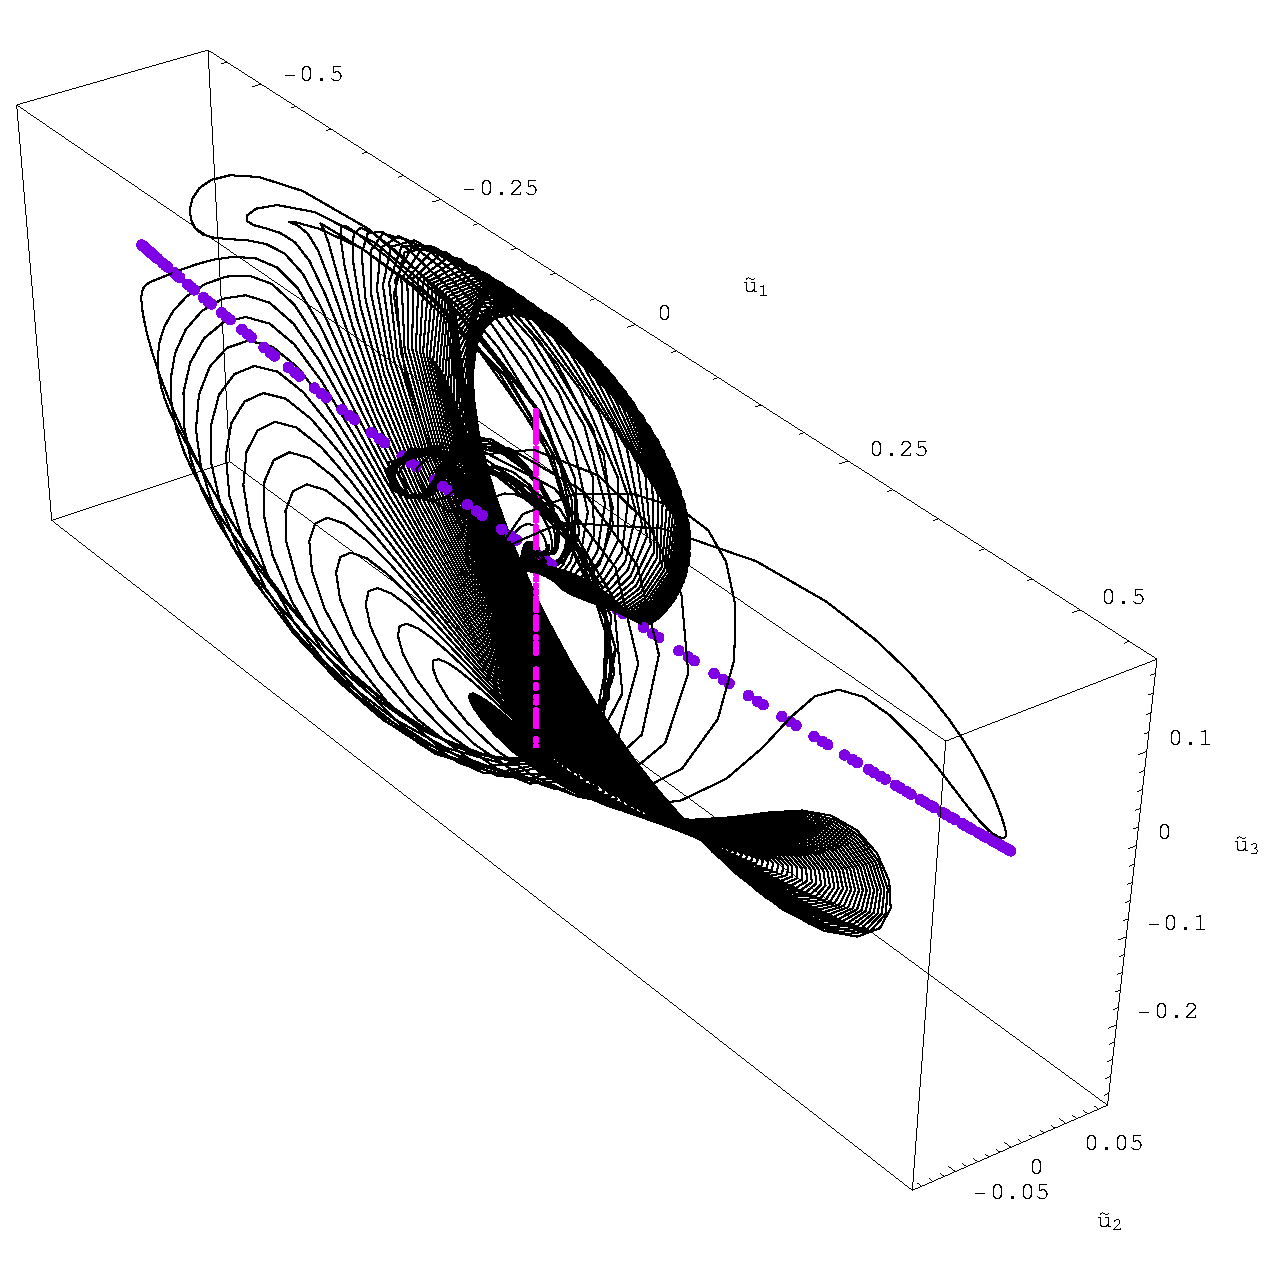
\includegraphics[width=5.0cm]{../figs/L22-2w-UnsMan.eps}
% \hspace{0.1in}
% (b) 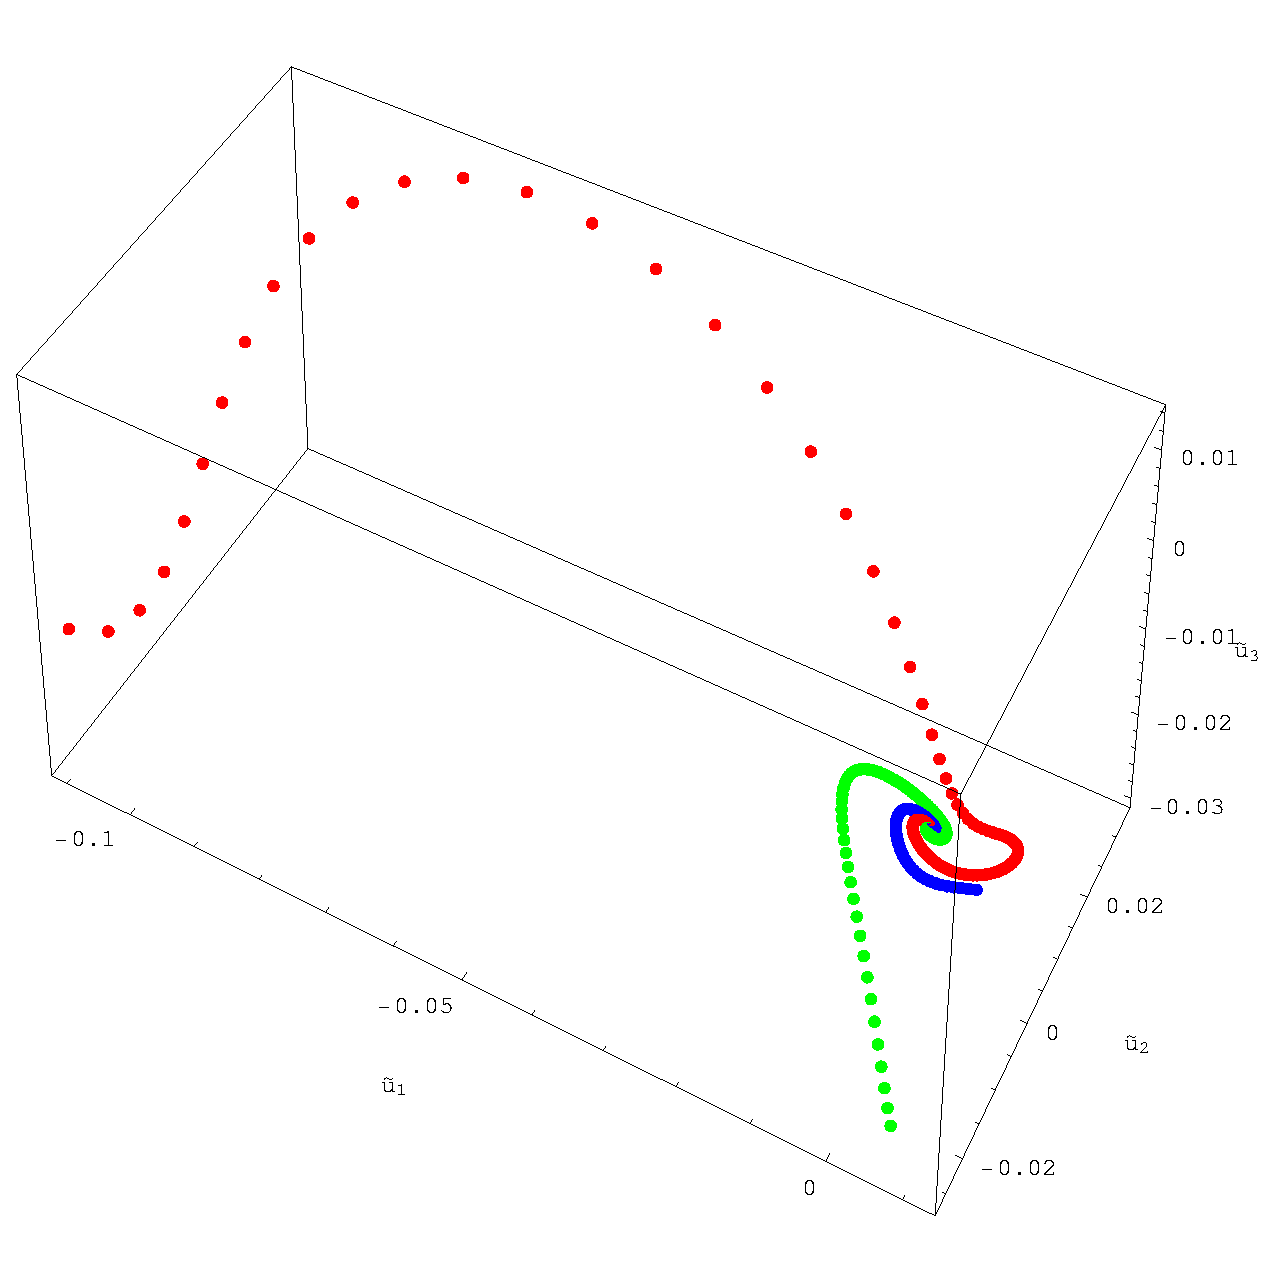
\includegraphics[width=5.0cm]{../figs/L22-2w-UnsMan-BlowUp.eps}
% % (b) 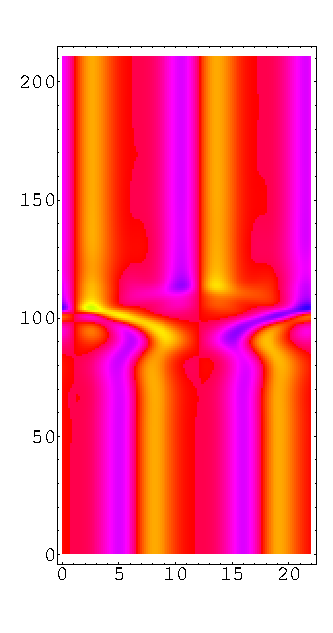
\includegraphics[width=4.0cm]{figs/L22-2w-R.eps}
% \\
% (c) 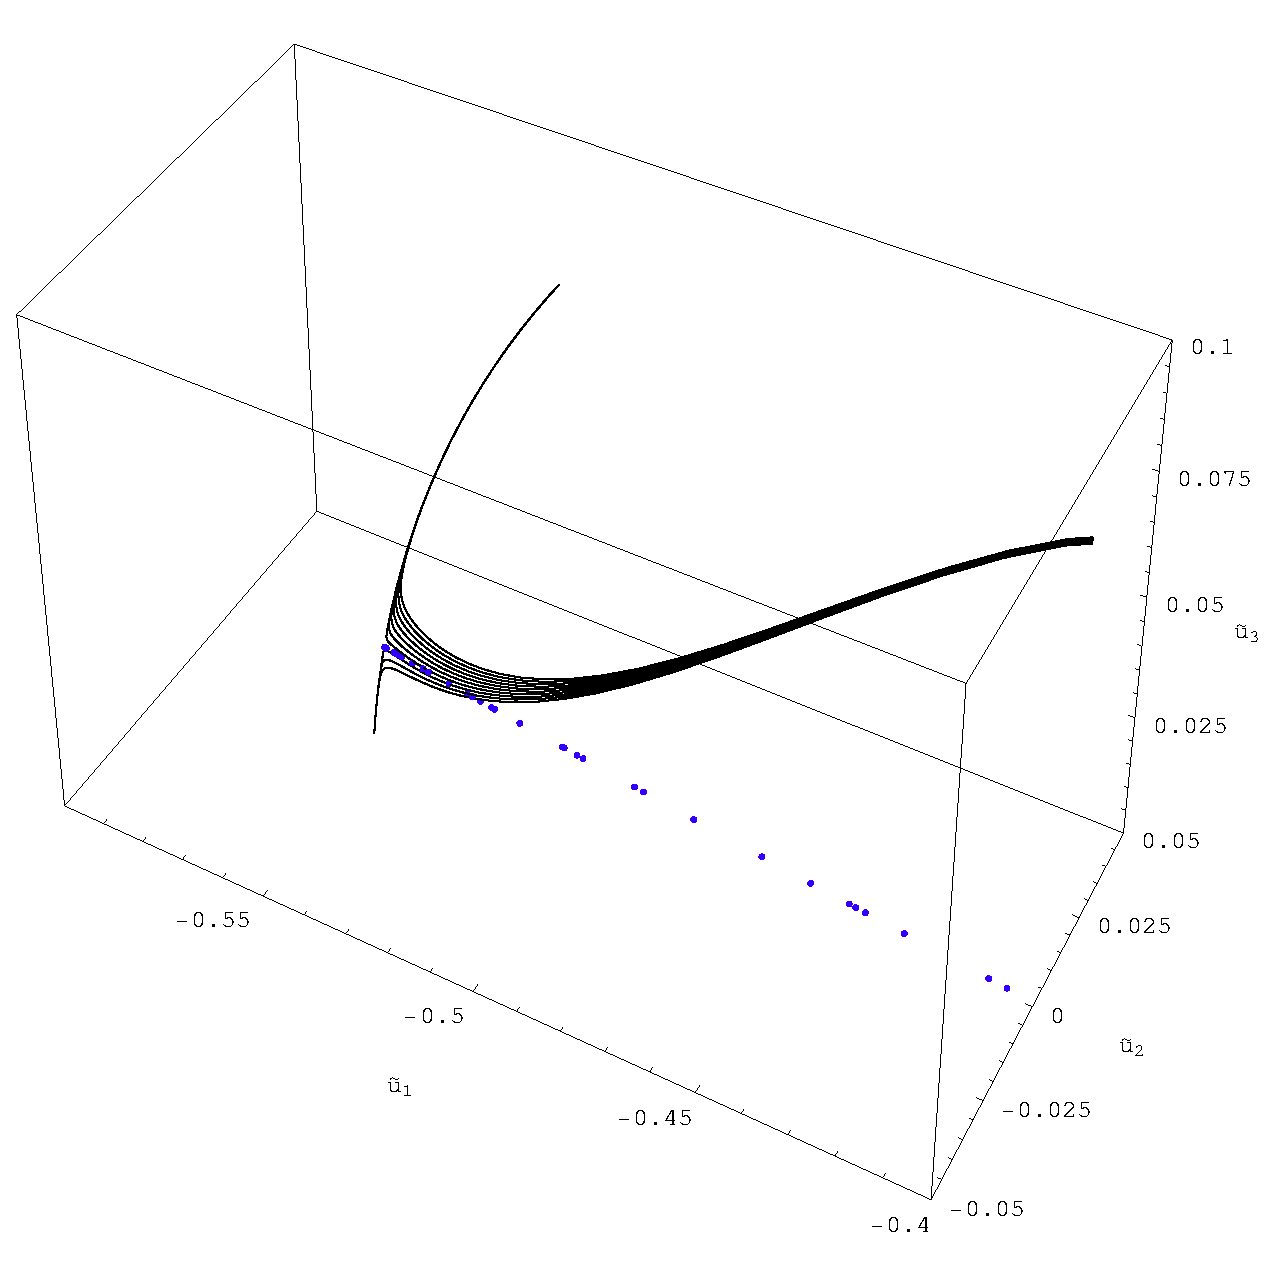
\includegraphics[width=5.0cm]{../figs/L22-2w-3w-UnsMan.eps}
% % (c) 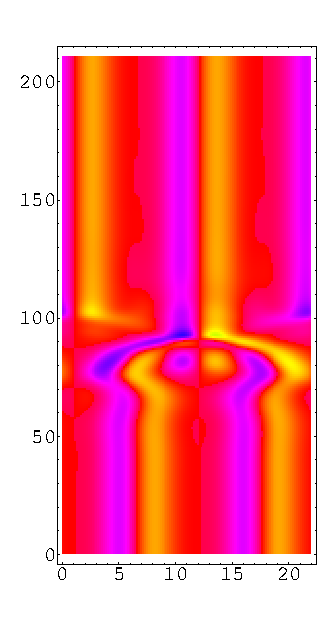
\includegraphics[width=4.0cm]{figs/L22-2w-G.eps}
% \hspace{0.1in}
% (d)  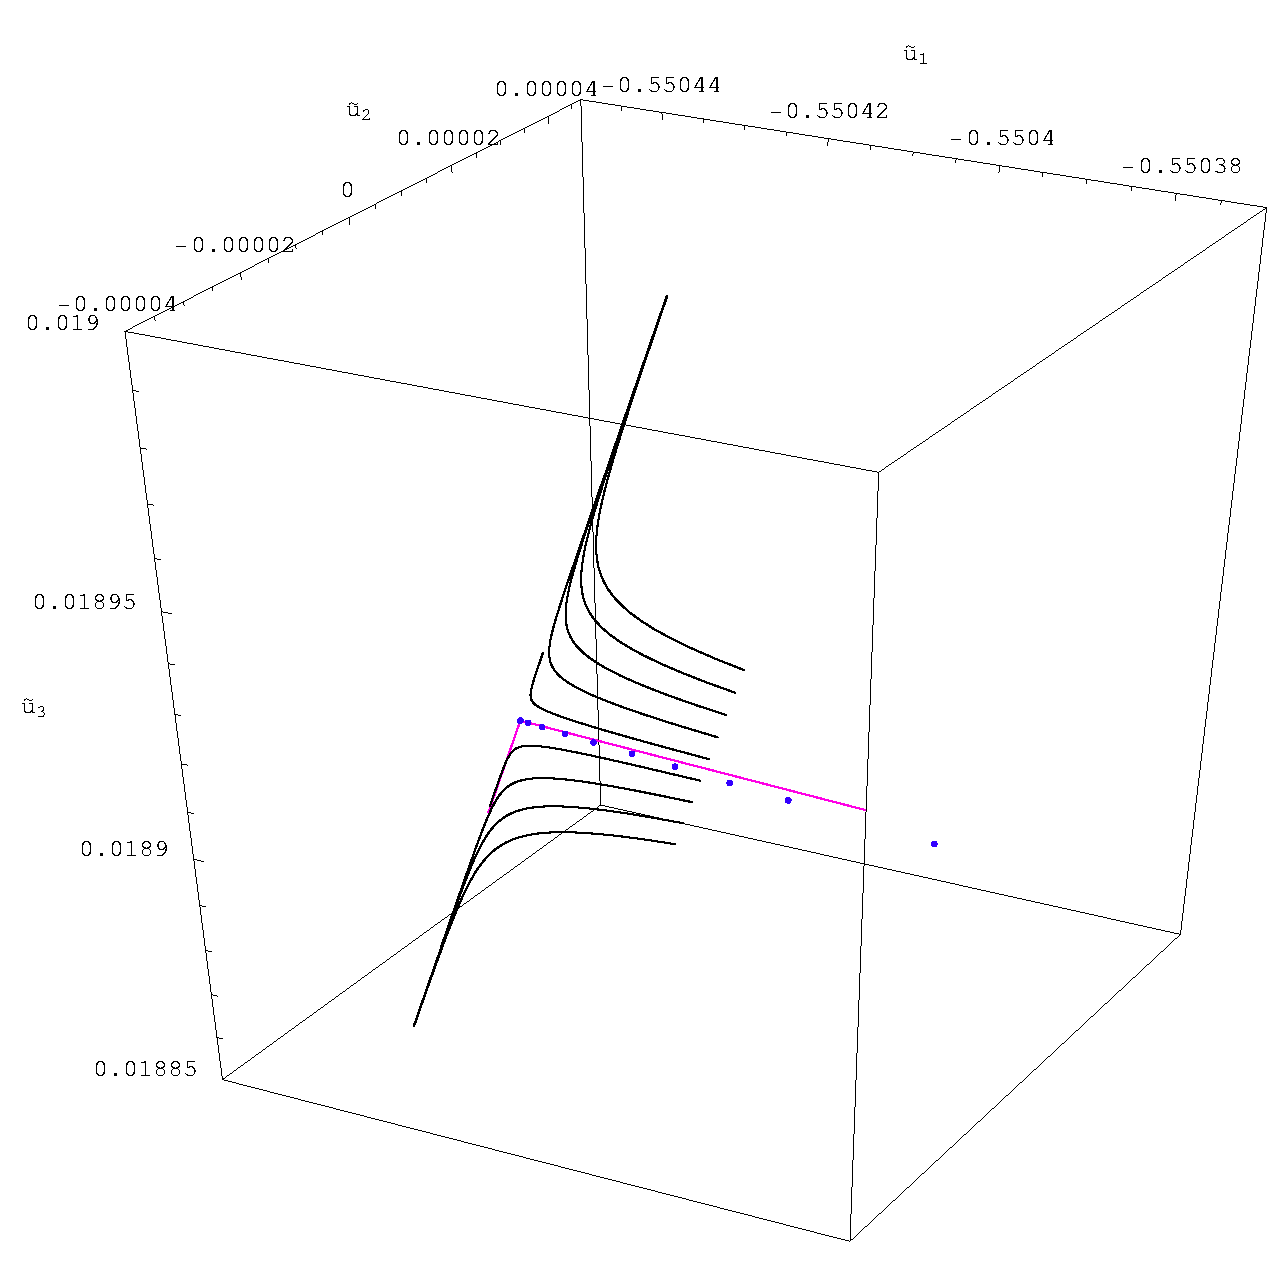
\includegraphics[width=5.0cm]{../figs/L22-2w-3w-detail.eps}
% % (d) 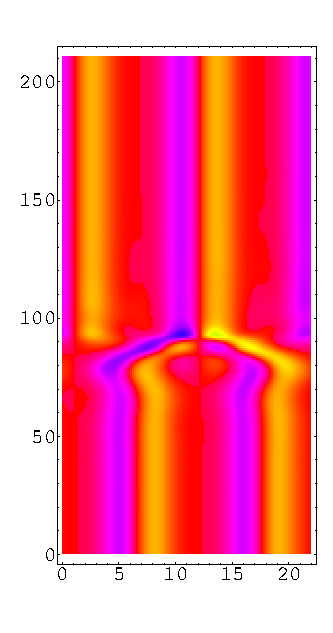
\includegraphics[width=4.0cm]{figs/L22-2w-B.eps}
% \end{center}
% \caption{
%  Trajectories with initial conditions on the unstable subspace of
%  the \EQV{2}~\eqv.
%  (a) The coordinates $\tilde{u}_1$ and $\tilde{u}_2$
%  are along the directions defining the unstable subspace
%  and $\tilde{u}_3$  is along the real part of the eigenvector
%  corresponding to the eigenvalue $-0.271122+ i\, 0.356307$.
% The purple points represent the continuous family
%  of
% \EQV{2}~\eqva.
% % Green curve belongs to \reffig{f:rpo55}(b) % rpo22-55-4-cm.eps
% % rather than to  \reffig{f:rpo55}(a), % rpoEq22-55-4.eps?
% (b) blowup of ``homoclinic'' descent of the unstable manifold
% back into \EQV{2}~\eqv, shifted by
% $L/4$.
% (c) blowup of ``heteroclinic'' connection from
% \EQV{2} \eqv\ to \EQV{3} \eqv, with shift
% $L(1/3-1/4) = L/12$
% \PCedit{(? check)}
% to the neighborhood of the point near which the
% unstable manifold of the
% \EQV{2} \eqv\ splits. The blue points
% represent the
% \EQV{3} {\eqv} family.
% The descent is along the eigenvector of $\Lyap_4= 0.413$,
% \ESedit{(checked)}
% and splitting
% occurs along one of the
% $\Lyap_1=\Lyap_2=0.0933$
% unstable directions of the \EQV{2}~{\eqv}.
% \ESedit{(checked)}
% (d) same as (c), closer to the \EQV{3}~{\eqv}.
% The eigendirections corresponding to $\Lyap_1$
% and $\Lyap_4$ are shown in purple.
% }
% \end{figure}
% %%%%%%%%%%%%%%%%%%%%%%%%%%%%%%%%%%%%%%%%%%%%%%%%%%%%%%%%%%%%%%%%%%
